\documentclass[aspectratio=169]{beamer}



\mode<presentation>
{
 \usetheme[reversetitle,notitle,noauthor]{Wien} 
%  \usetheme[noauthor]{Wien} 
}       
  
\usepackage{url}
\usepackage{graphicx}
\graphicspath{{./}{./Figures/}}  
\usepackage{graphicx}
\usepackage{appendixnumberbeamer} 
\usepackage{movie15}
% To avoid a warning from the hyperref package:
\pdfstringdefDisableCommands{%
  \def\translate{}%
}

% To make sure, that the footnote is placed above and outside the
% footline (but it only works for one footnote per frame):
% 
% \addtobeamertemplate{footnote}{}{\vspace{4ex}}

%%%%%%%%%%%%%%%%%%%%%%%%%%%%%%%%%%%%%%%%%%%%%%%%%%%%%%%%%%%%%%%%%%%%%%%%%%%%% 
%%%%%%%%%%%%%%%%%%%%%%%%%%%%%%%%%%%%%%%%%%%%%%%%%%%%%%%%%%%%%%%%%%%%%%%%%%%%%
\title[ICT Presentations]{Autoroutes du Sud-Ouest de la France }

\subtitle{Groupe 7}



\institute[TU Wien]{FDS Montpellier}
   
\date{Le 13 Décembre 2021}

\author[A. Jantsch]{ABDERRAHIM AIT MOULAY \\ ADRIEN SIMON \\ ASSANE SENE}

\begin{document}

\begin{frame}
  \titlepage
\end{frame}      

%%%%%%%%%%%%%%%%%%%%%%%%%%%%%%%%%%%%%%%%%%%%%%%%%%%%%%%%%%%%%%%%%%%%%%%%%%%%% 
%%%%%%%%%%%%%%%%%%%%%%%%%%%%%%%%%%%%%%%%%%%%%%%%%%%%%%%%%%%%%%%%%%%%%%%%%%%%%
%%%%%%%%%%%%%%%%%%%%%%%%%%%%%%%%%%%%%%%%%%%%%%%%%%%%%%%%%%%%%%%%%%%%%%%%%%%%%

\begin{frame}{Plan}
  

   \begin{enumerate}
       \item Introdution 
       \item Nettoyage de données 
       \item La carte interactive
       \item Programme d'optimisation
       \item KDE de la distribution des prix par kilomètre
       \item Conclusion 
       
   \end{enumerate}


\end{frame}

%%%%%%%%%%%%%%%%%%%%%%%%%%%%%%%%%%%%%%%%%%%%%%%%%%%%%%%%%%
%%%%%%%%%%%% Introduction %%%%%%%%%%%%%%%%%%%%%%%%%%%%%%%%

\begin{frame}{Introduction}

\begin{block}{Répartition du travail}
 \begin{itemize}
    \item Abderrahim s'est occupé de la carte interractive, du nettoyage de la base de données des distances et de la mise en place de la documentation
    \item Assane s'est occupé de la répartition des prix et du nettoyage de la base de donnée des prix
    \item Adrien s'est occupé de la minimisation du coût du trajet et du calcul des distances à partir des coordonnées GPS
    
\end{itemize}
\end{block}
    
\end{frame}


%%%%%%%%%%%%%%%%%%% Nettoyage de données %%%%%%%%%%%%%%%%%%%%%%%%%%%%%%%%%%%%%%%%

\begin{frame}{Nettoyage de données}
\begin{block}{Creation dataframe et matrice prix}
 \begin{itemize}
\item Importation des données avec la fonction \textbf{pd.read\_csv()}:\\[2 mm]
df\_p = pd.read\_csv("Data\_prix.csv").\\[2 mm]
\item Remplacement des NAN par 0.0 dans le dataframe:\\
df\_p = df\_p.fillna(0.0).\\[2 mm]
\item suppression des colonnes (ou des sorties) où l'on ne peut pas sortir:\\[2 mm]
Avec la fonction \textbf{del}, nous allons supprimer les sorties auxquelles on ne peut pas sortir. Ces dernières sont:
\begin{itemize}
\item Peage de Montpellier St-Jean
\item Peage du Perthus
\item Le Boulou (peage sys ouvert)
\item Peage de pamiers
\item Peage de Toulouse sud/ouest
\item Peage de Toulouse sud/est

\end{itemize}    
\end{itemize}  
\end{block}
  
\end{frame}    

\begin{frame}{Nettoyage de données}
\begin{block}{}
 \begin{itemize}
\item remplacement de 0 par 0.0 et 8.58,5 par 8.5 dans les colonnes Vendargues et Narbonne sud du dataframe et affichage du nouveau dataframe:\\[2 mm]

\item transformation du dataframe df\_p en matrice (numpy array):\\[2 mm]
df\_pnmp = np.array(df\_p, dtype = 'float64')
\end{itemize}
\end{block}

\end{frame}





%%%%%%%%%%%%%%%%%%%%%%% Carte interactive %%%%%%%%%%%%%%%%%%%%%%%%%%%%%%%%%%%%%%%

\begin{frame}{La carte interactive}

\begin{block}{Objectif}
 L’objectif principal de cette partie est de créer une carte interactive avec le package {\color{blue} folium} afin d’afficher l’itinéraire, la distance, le prix ainsi que le prix par kilomètre entre deux gares données par l’utilisateur.

\end{block}
\pause
\begin{block}{Fonction}

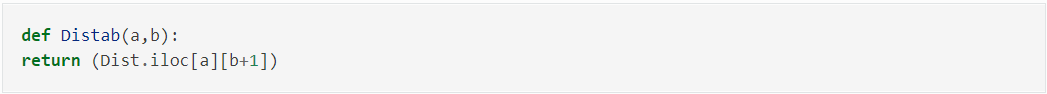
\includegraphics[scale=0.7]{1.png}
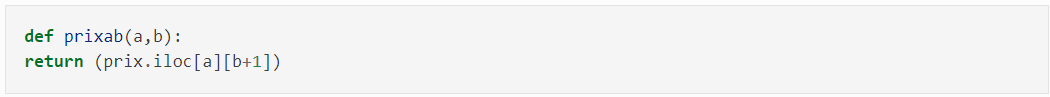
\includegraphics[scale=0.7]{2.png}

\end{block}
\end{frame}
\begin{frame}{La carte interactive}
Nous avons utiliser la fonction "folium.map" qui nous permet d'afficher une carte vide.
 \begin{block}{}
       {\color{blue}folium.Map(location=.....,zoom\_start=....., control\_scale=....)} 
 \end{block} 
 
 \begin{center}
  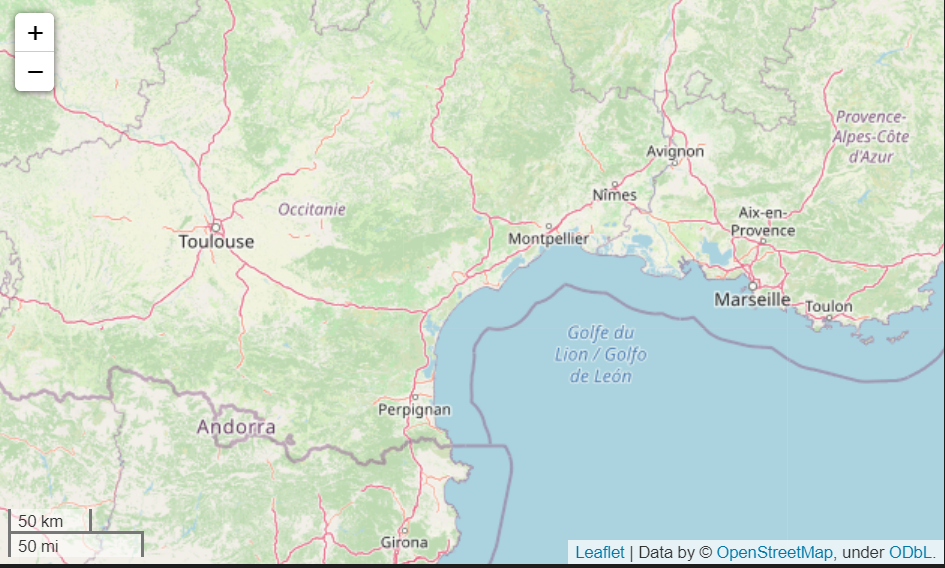
\includegraphics[scale=0.5]{Carte_vide.png}
 \end{center}
    
\end{frame}

\begin{frame}{La carte interactive}
Pour afficher un point sur la carte nous avons utiliser la fonction "folium.Marker".

 \begin{block}{}
  {\color{blue}folium.Marker( location=list(.......),  ).add\_to(m)} 
 \end{block} 

 \begin{center}
  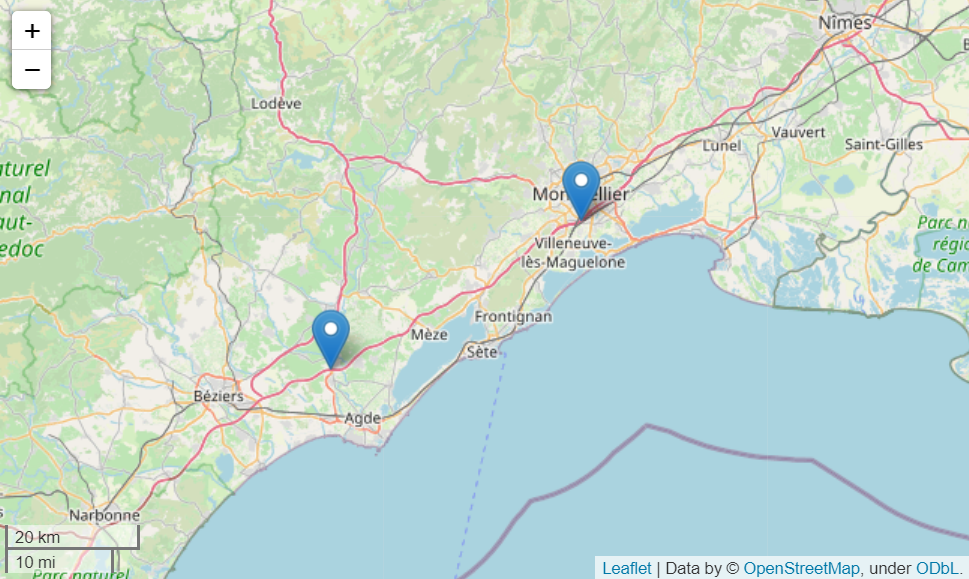
\includegraphics[scale=0.5]{Carte_2_point.png}
 \end{center}
\end{frame}

\begin{frame}{La carte interactive}
Pour tracer la route entre des points donnés nous avons utiliser la fonction "folium.GeoJson".
 \begin{block}{}
  {\color{blue}geometry = client.directions(coords)['routes'][0]['geometry']
 decoded = convert.decode\_polyline(geometry)
 folium.GeoJson(decoded).add\_child(folium.Popup(max\_width=300)).add\_to(m)} 
 \end{block} 
 
 \begin{center}
  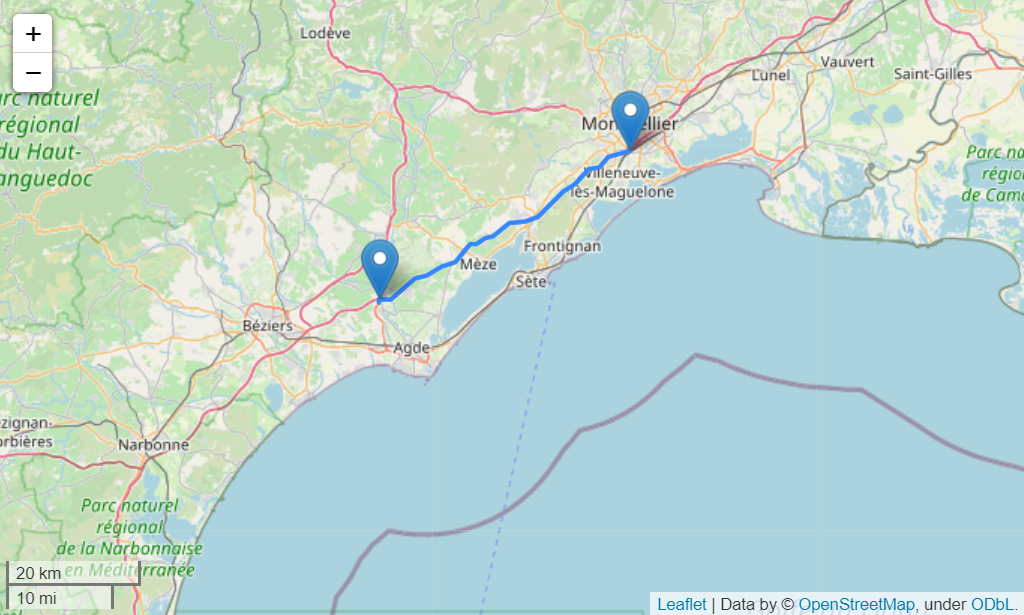
\includegraphics[scale=0.4]{Carte_iti.png}
 \end{center}
\end{frame}

\begin{frame}{La carte interactive}
Pour ajouter le texte de la fenêtre contextuelle lorsque nous cliquons sur l’itinéraire.

 \begin{block}{}
  {\color{blue} folium.GeoJson(decoded).add\_child(folium.Popup(texte,max\_width = 300)).add\_to(m)} 
 \end{block} 

\begin{center}
 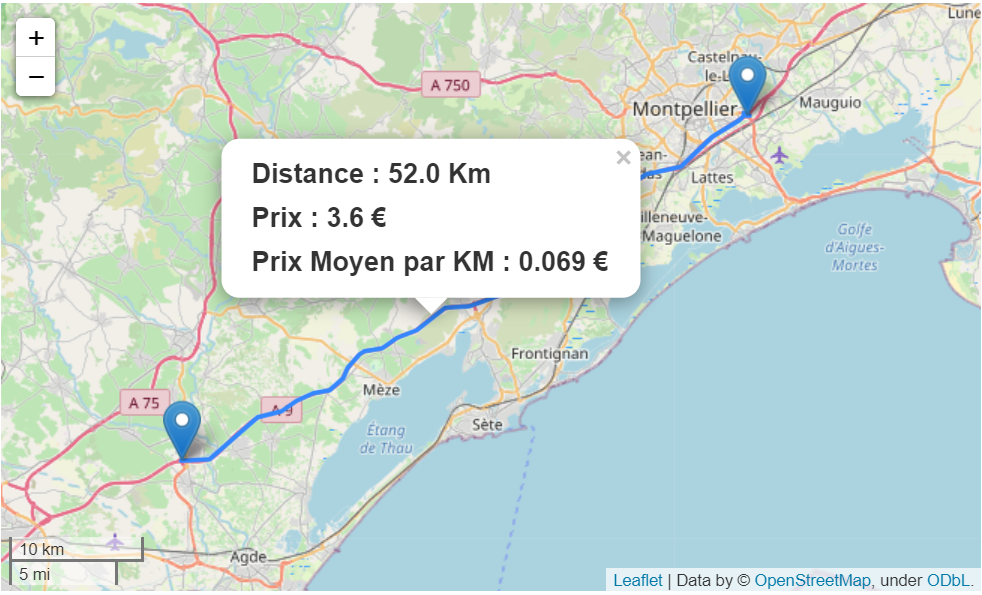
\includegraphics[scale=0.5]{Carte_prix_dist.png}
\end{center}
\end{frame}

\begin{frame}{Widgets}

 \begin{block}{}
  {\color{blue} interact(itineraire, DEPART = villes, ARRIVEE = villes) } 
 \end{block} 

\begin{center}
 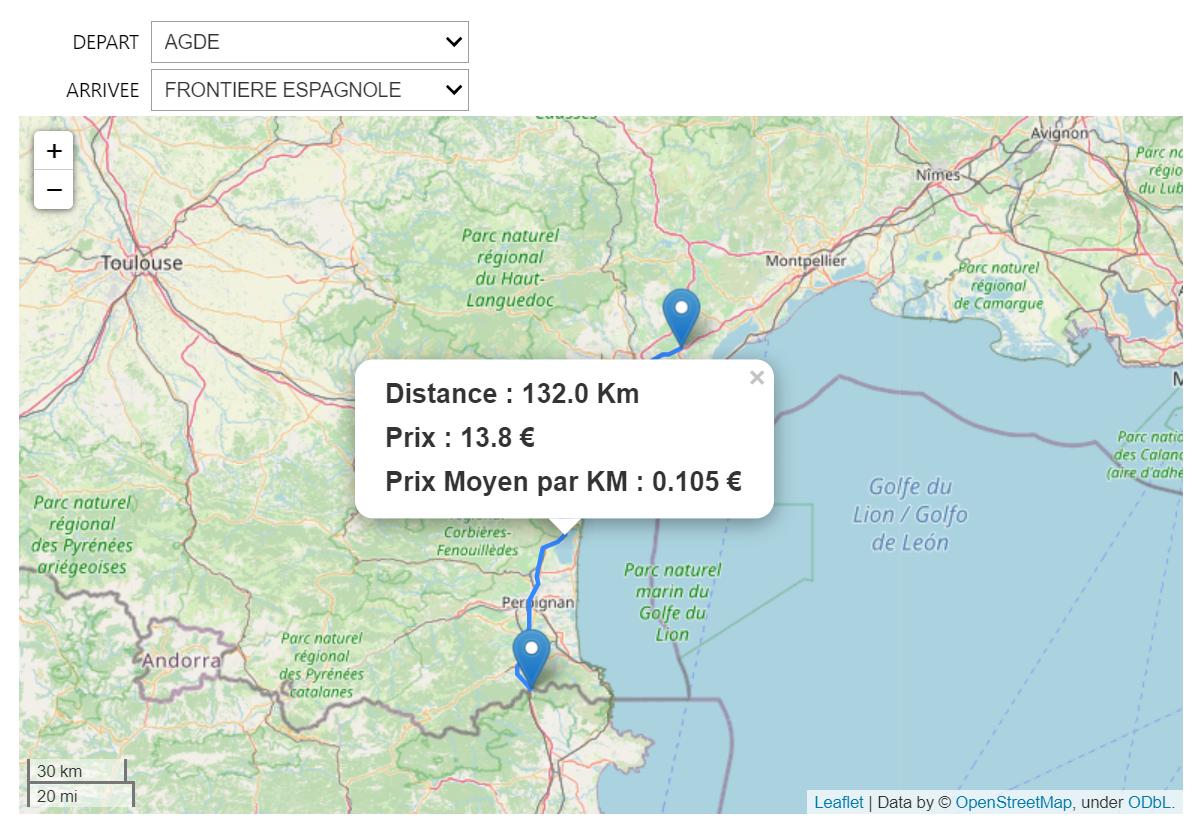
\includegraphics[scale=0.45]{Carte-1.png}
\end{center}
\end{frame}
%%%%%%%%%%%%%%%%%%%%%%%%%%%%%%%%%%% Programme d'optimisation %%%%%%%%%%%%%%%%%%%%%%%%%
\begin{frame}[fragile]{Programme d'optimisation}
  
\begin{block}{Rappel de l'objectif}

Le but de cette partie est de minimiser le coût du trajet selon un nombre de sorties intermédiares maximum donné. 
\end{block}

\end{frame}

\begin{frame}[fragile]{Processus de résolution}
\begin{block}{Etapes intermédiaires}
 

\begin{itemize}
    \item Comment ordonner les sorties ?
    \item Comment faire pour obtenir toutes les combinaisons de n sorties entre deux points sur l’autoroute ?
    \item Comment traiter les sorties "problématiques" ?
    \item Comment fonctionne l’algorithme et comment pourrait-on l’optimiser ?
\end{itemize}

\end{block}

\end{frame}

\begin{frame}{Passer d'un système sans ordre à un système ordonné}

\begin{center}

    \includegraphics[scale=0.4]{Carte.png}
    \begin{tabular}{*{4}{|c|}}
   \hline
   Portion 1 & Vendargues & ... & Narbonne Sud \\
  \hline
    Portion 2 & Sigean & ... & Frontière Espagnole \\
  \hline
  Portion 3 & Lezignan & ... & Villefranche-de-Lauragais \\
  \hline
  Portion 4 & Nailloux & ... & Pamiers Sud\\
  \hline
  Portion 5 & Montgiscard & ... & Sesquières \\
  \hline
\end{tabular}
\end{center}



\end{frame}

\begin{frame}{Utilisation de itertools}

\begin{block}{ Fonction itertools.combinations}
J'ai combiné la fonction combinations de la librairie itertools avec ma fonction nbSorties pour obtenir la fonction que j'ai nommée march()
\end{block}

\begin{center}
 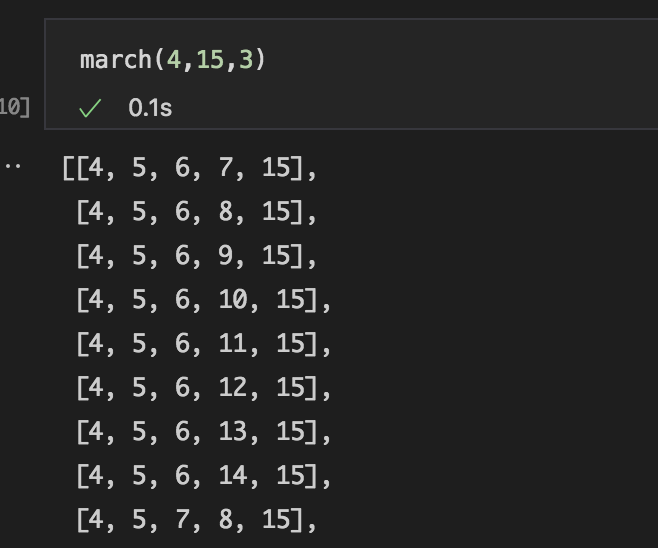
\includegraphics[scale=0.45]{fct march.png}
\end{center}


\end{frame}

\begin{frame}{Sorties à problèmes}

\begin{block}{traiter les cas particuliers}
Pourquoi as-t-on décidé de ne pas prendre en compte les peages ?

Comment faire pour contourner les problèmes posés par les sorties Le boulou sur la A9 et Pamiers Nord sur la A66 ?
 
\end{block}
    
\end{frame}

\begin{frame}{Fonctionnement global et optimisation du code}
    \begin{block}{fonctionnement de base}
     Combiner la fonction Finale() et l'utilisation de widgets
    \end{block}
    \begin{center}
            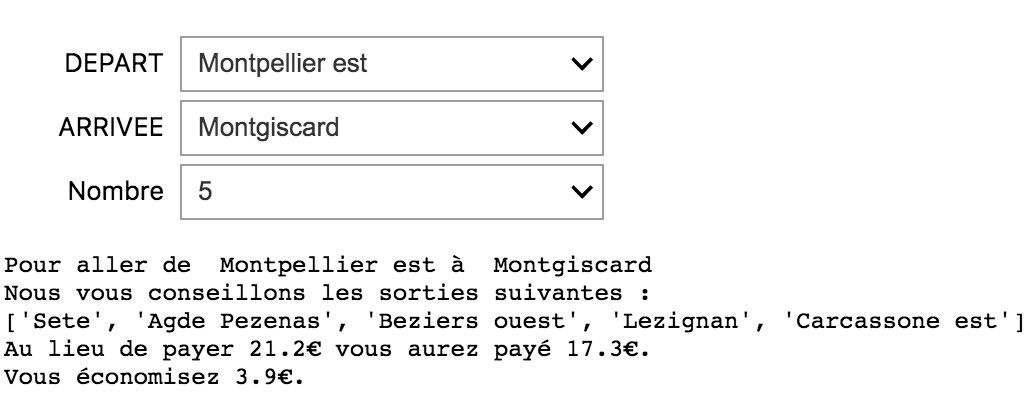
\includegraphics[scale=0.45]{fctFinale1.png}

    \end{center}
\end{frame}

\begin{frame}{Fonctionnement global et optimisation du code (suite)}
\begin{block}{NetworkX et graphs}
    Autres méthodes pour la partie de minimisation du prix du trajet : Les graphs et l'algorithme de Kruskal
    \end{block}
    \begin{block}{Optimisation du code}
     Comment pourrait-on réduire les temps de calcul en conservant notre méthode de résolution de la problématique ?
    \end{block}
\end{frame}

%%%%%%%%%%%%%%%%%%%%%%% KDE %%%%%%%%%%%%%%%%%%%%%%%%%%%%%%%%%%%%%%%

\begin{frame}{KDE de la distribution des prix par kilomètre}
\begin{block}{Objectif }
 Dans cette partie, nous allons essayer de donner un KDE (distribution, estimation, tracer de courbe, ...) des prix par km entre une entrée et une sortie choisies, à l'aide de fonction interact contenue dans le module ipywidgets. Dans un premier temps, nous allons faire un nettoyage des données. Puis , nous créerons un data frame des prix par km. Enfin,nous ferons un KDE de ce data frame obtenu.
\end{block}
    
\end{frame}



\begin{frame}{KDE de la distribution des prix par kilomètre}
\begin{block}{Création des fonctions}
\begin{itemize}
\item def Distribution\_Prix(i,j):\\[2 mm]
Cette fonction calcule le prix entre toutes les sorties successives parmi toutes les sorties qui se trouvent entre i et j. \\[2 mm]
\item def Distribution\_dist(i,j):\\[2 mm]
Cette fonction calcule la distance entre toutes les sorties successives parmi toutes les sorties qui se trouvent entre i et j. \\[2 mm]
\end{itemize}
\end{block}
\end{frame}
\begin{frame}{KDE de la distribution des prix par kilomètre}
\begin{block}{Fonctions}
 \begin{itemize}

\item def moyDist(i,j):\\[2 mm]
Cette fonction permet de calculer la prix par km entre toutes les sorties successives parmi toutes les sorties qui se trouvent entre i et j.\\[2 mm]
\item creation du vecteur villes:\\
villes = []...\\
\end{itemize}
\end{block} 

\end{frame}

\begin{frame}{KDE de la distribution des prix par kilomètre}
\begin{block}{}
 interact(kde\_explore, entre = villes, sortie = villes, bw = (0.001, 2, 0.01))\\[2 mm]
\end{block}
\begin{center}
 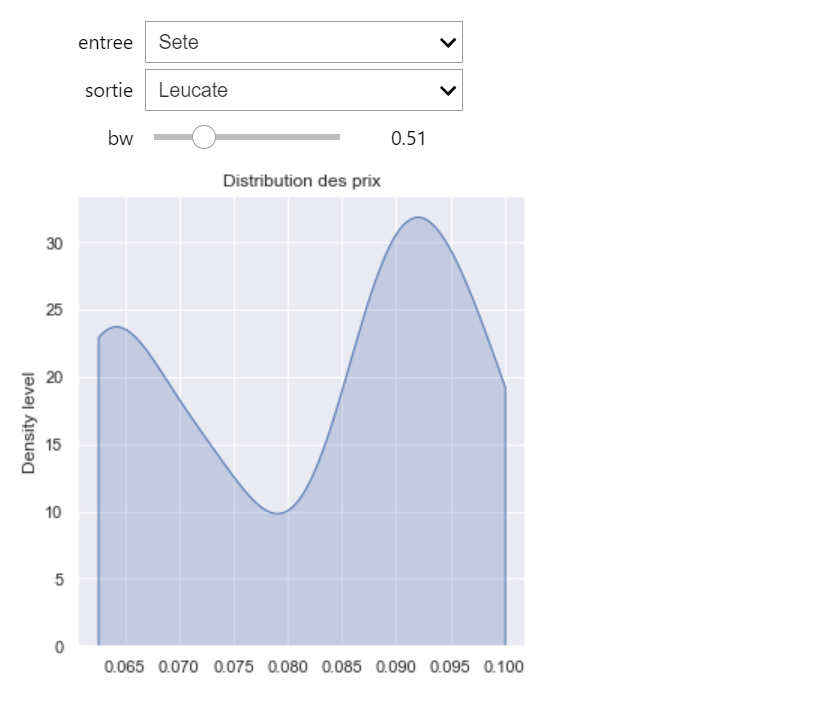
\includegraphics[scale=0.55]{KDE1.png}
\end{center}

\end{frame}
%%%%%%%%%%%%%%%%%%%%% Conclusion %%%%%%%%%%%%%%%%%%%%%%%%%%%%%%%%%

\begin{frame}{Conclusion}
    \begin{block}{le programme asof.py}
    Nous avons finalement combiné l'ensemble de notre travail dans un seul fichier python qui appelle les trois parties de ce projet et qui permet d'avoir l'affichage de la carte interractive, le trajet le moins cher sur une section d'autoroute et la répartition des prix. Il suffit d'executer le fichier asof.py et de choisir les sorties qui vous intéressent dans les widgets interractifs !
    
    \end{block}
    
    
    
\end{frame}




%%%%%%%%%%%%%%%%%%%%%%%%%%%%%%%%%%%%%%%%%%%%%%%%%%%%%%%%%%%%%%%%

\begin{frame}{}

 \begin{block}{}
  $ \;\;\;\; \; $ \\
  \begin{center}
      MERCI POUR VOTRE ATTENTION !! \\
  \end{center}
   
   $\;\;\;$ \\
 \end{block}
    
\end{frame}



\end{document}


%%% Local Variables:
%%% mode: latex
%%% TeX-master: t
%%% End:
